\chapter*{\thechapter \quad Git}
\addcontentsline{toc}{chapter}{\thechapter \quad Git}
\paragraph{}

Esta secção tem o objetivo de demonstrar a lógica utilizada na plataforma \textit{GIT} para o desenvolvimento deste relatório, é possivel aceder ao repositório através do \textit{link} referenciado na bibliografia.

Para o desenvolvimento do relatório utilizamos a seguinte metodologia:
\begin{itemize}
    \item Inicialmente foi criada a estrutura de grande parte do projeto por parte do responsável de repositório e esta foi colocada disponivel no ramo principal do repositório;
    \item Desse ponto em diante foi utilizada sempre a mesma lógica por parte dos contribuidores:
    \begin{itemize}
    \item Todos os contribuidores fazem o clone do projeto para os seus computadores.;
    \item Criação de um \textit{branch};
    \item Alterações do conteúdo no respetivo \textit{branch};
    \item \textit{Commit} e \textit{push} para o \textit{branch} das alterações feitas;
    \item Criação de um \textit{pull request} do \textit{branch} criado para o principal;
    \end{itemize}
    
    \item Para a aprovação de um \textit{pull request} é necessário:
    \begin{itemize}
    \item Aprovação por parte dos contribuidores;
    \item Aprovação e \textit{merge} por parte do responsável do repositório;
    \end{itemize}
\end{itemize}

\begin{table} 
\begin{center}
\begin{tabular}{||c c||} 
 \hline
 Responsáveis de repositório & Contribuidores  \\ [0.5ex] 
 \hline\hline
 António Ferreira & António Ferreira \\ 
 \hline
  & Diogo Miranda \\
 \hline
  & Pedro Meneses \\
 \hline
  & Ricardo Fernandes \\ [1ex] 
 \hline
\end{tabular}
\caption{Tabela de responsabilidades}
\label{table: Tabela de responsabilidades}
\end{center}
\end{table}

\newpage

As figuras seguintes ilustram o trabalho desenvolvido no repositório:

\begin{figure}[H]
	\begin{center}
		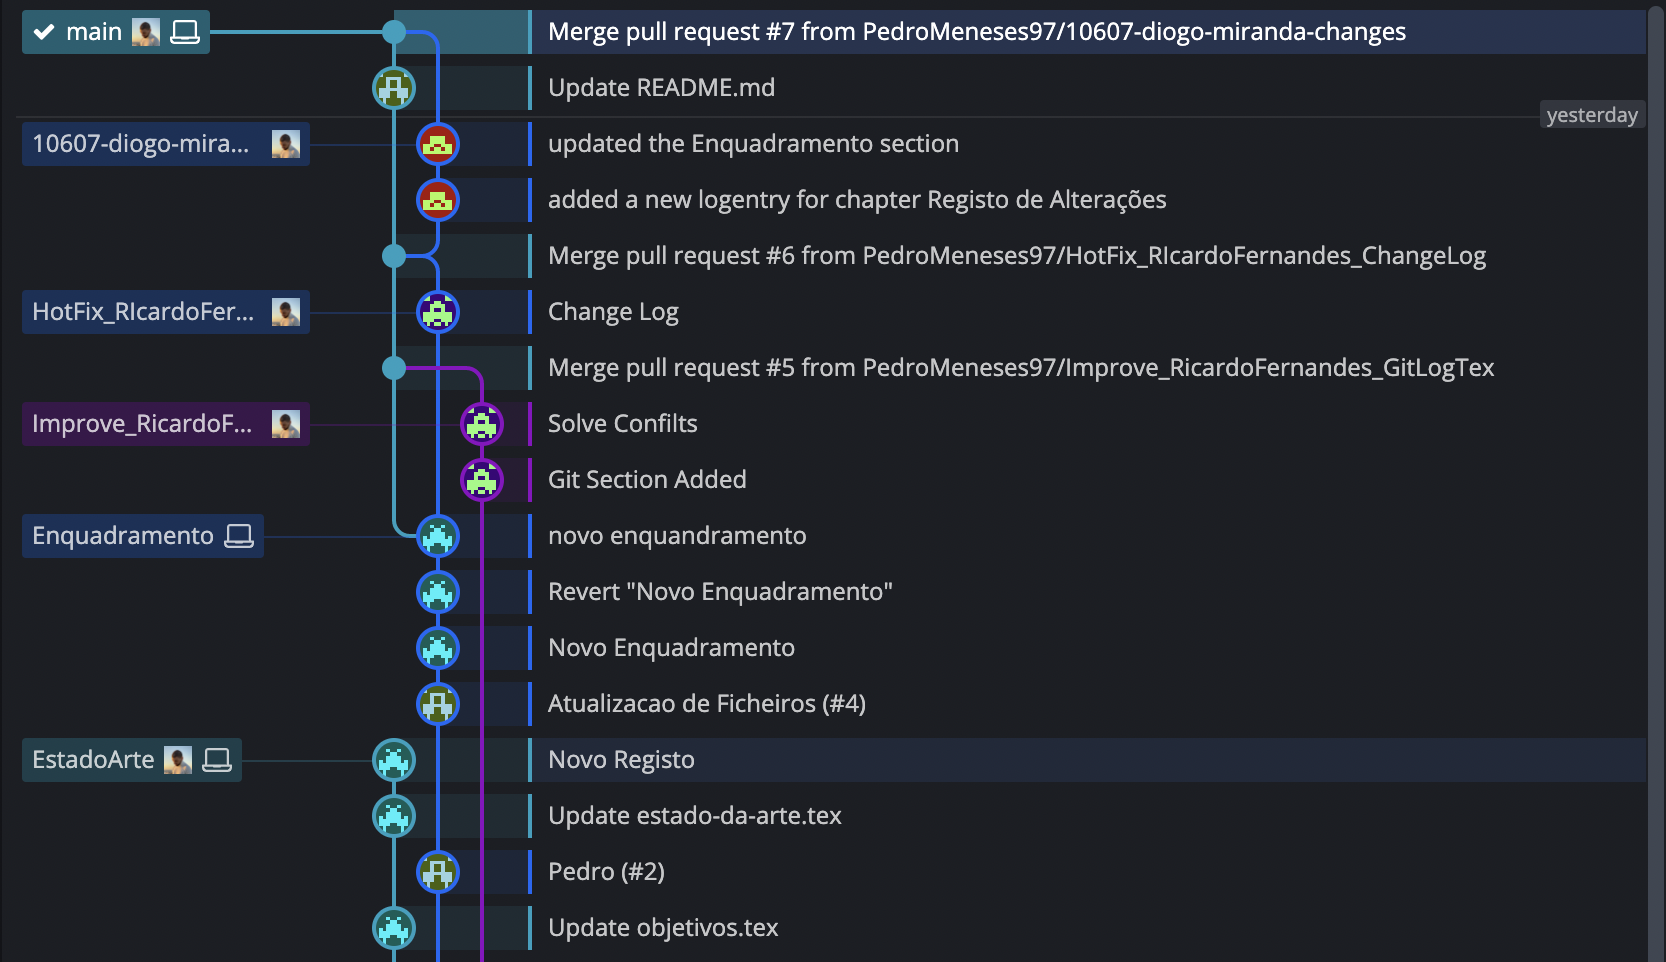
\includegraphics[width=1.0\textwidth]{chapter/image/git1.png}
	\end{center}
		\caption{Figura \textit{GIT} A}
		\label{fig:git-pica}
\end{figure}



\begin{figure}[H]
	\begin{center}
		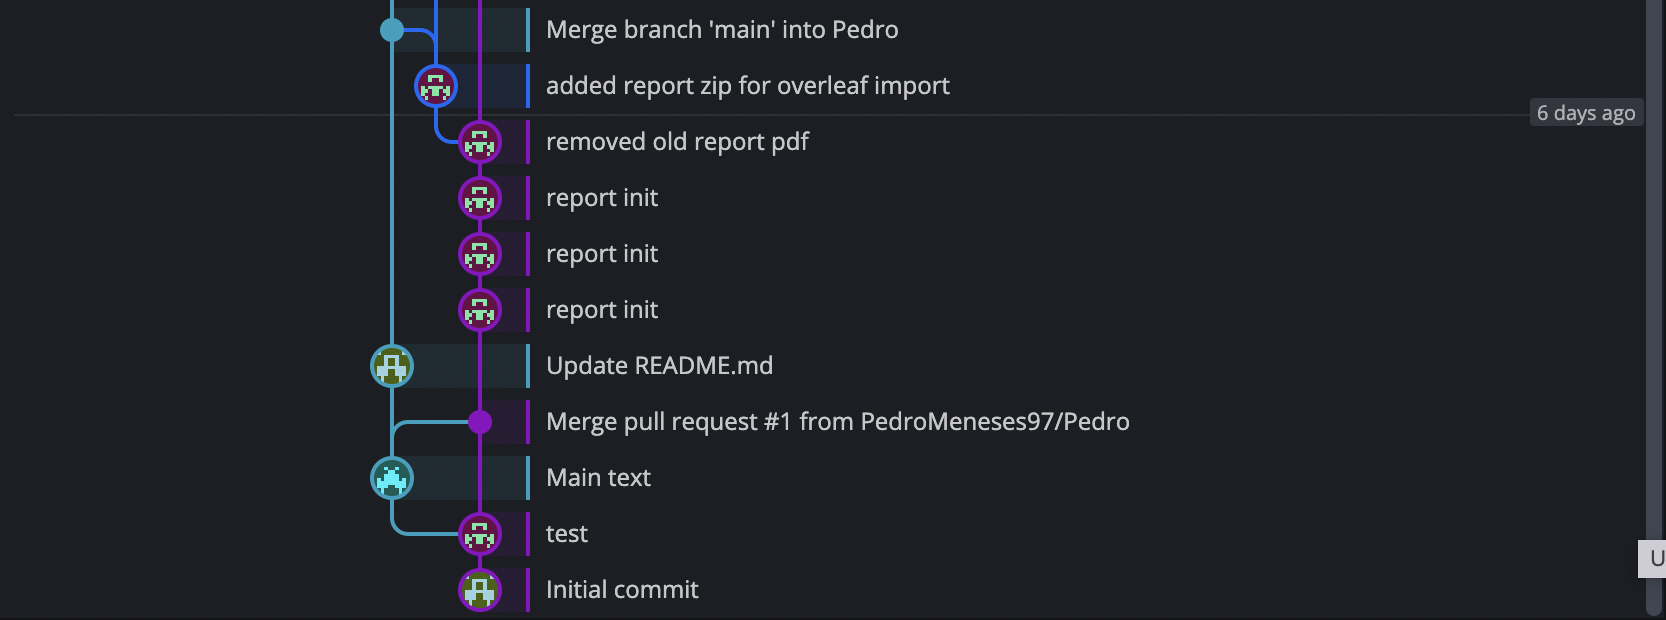
\includegraphics[width=1.0\textwidth]{chapter/image/git2.png}
	\end{center}
		\caption{Figura \textit{GIT} B}
		\label{fig:git-picb}
\end{figure}



\begin{figure}[H]
	\begin{center}
		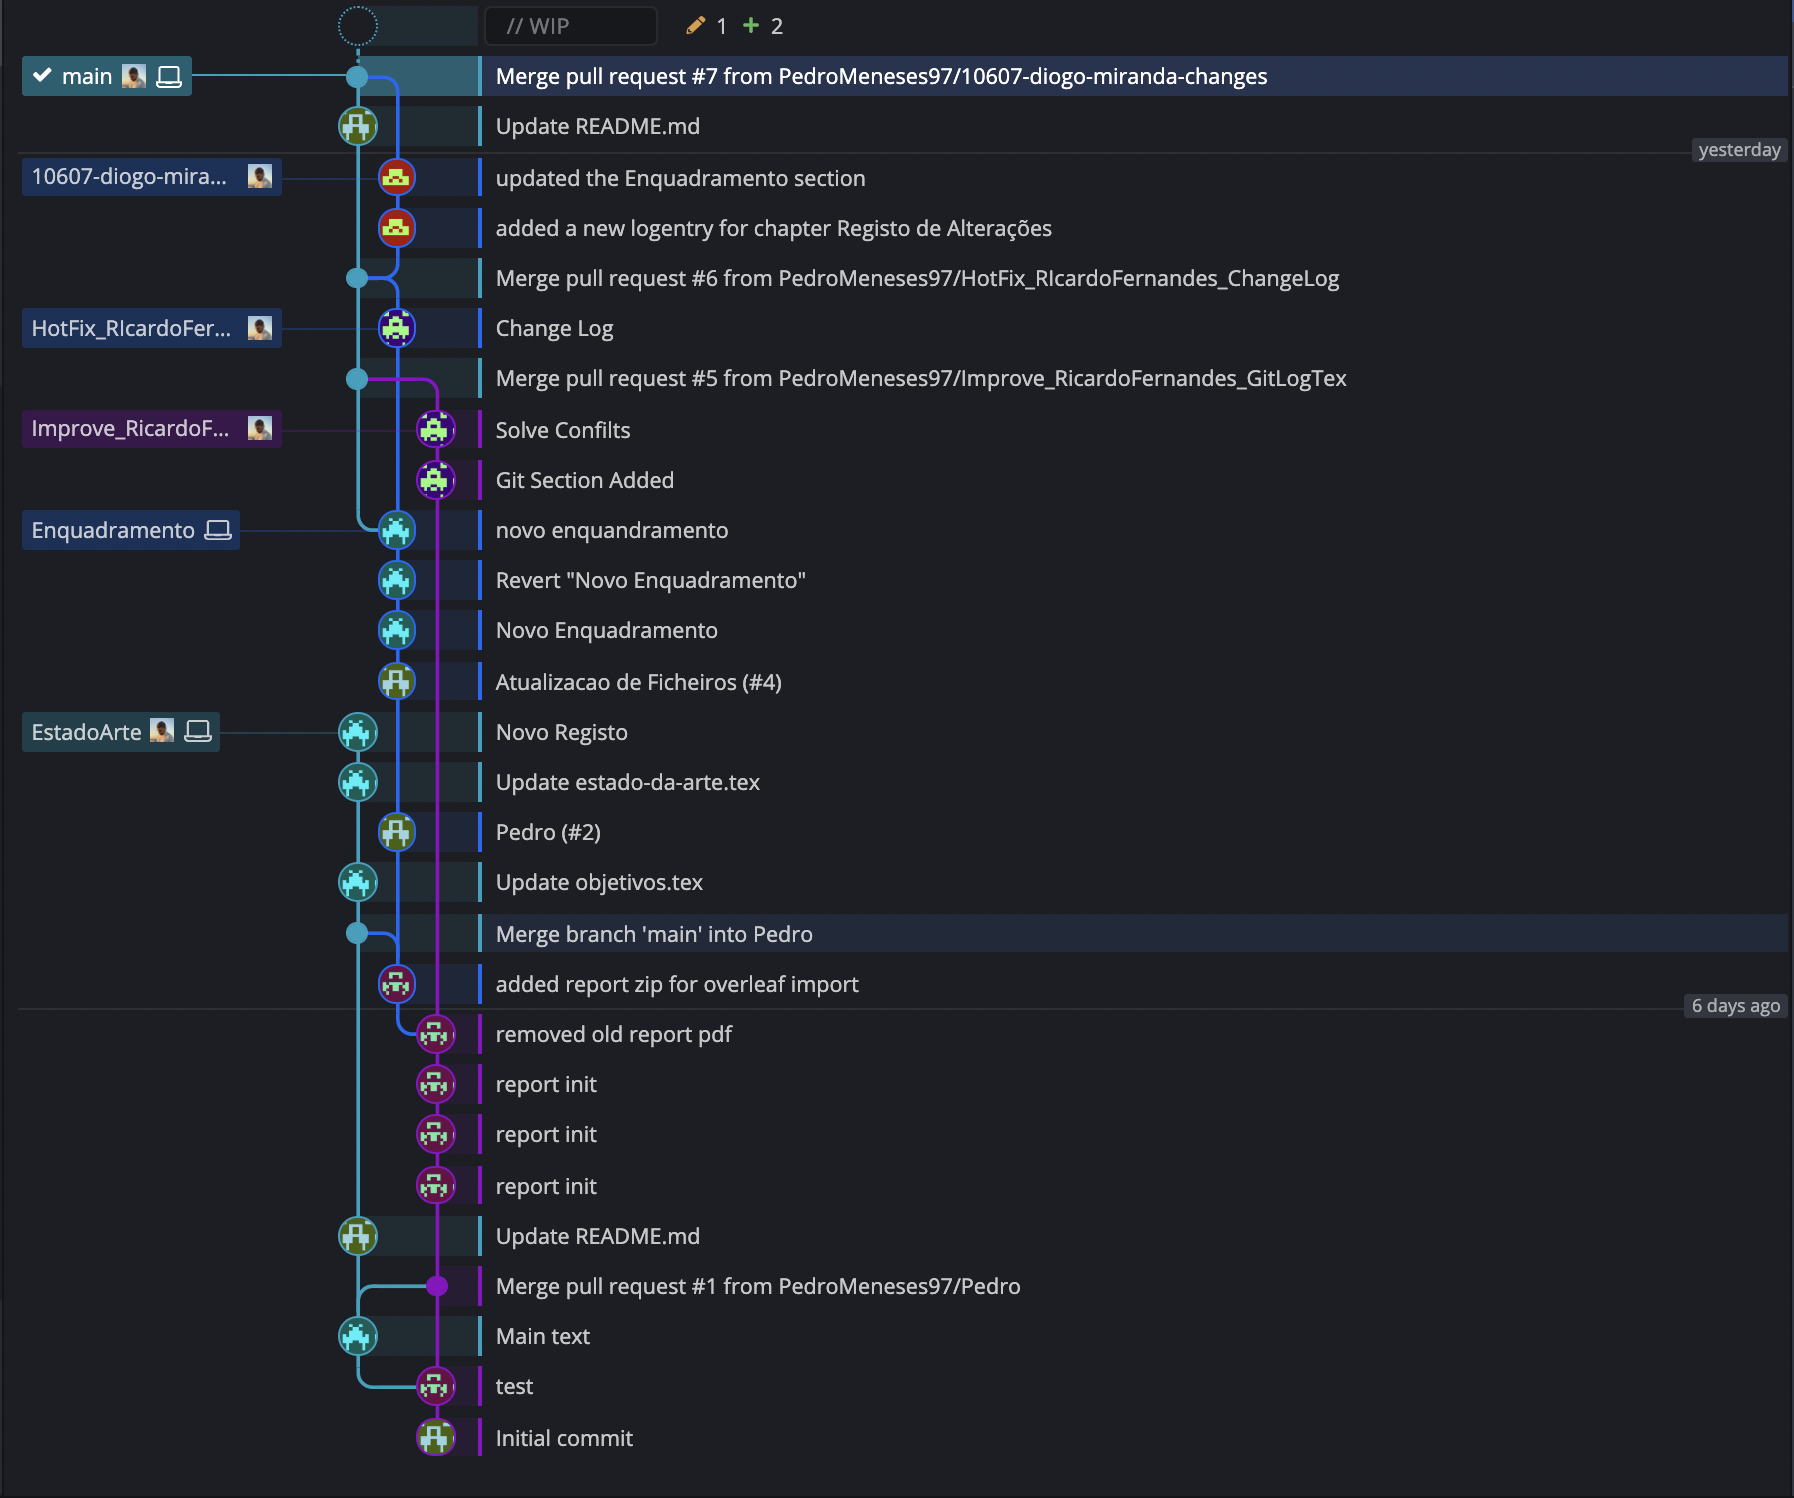
\includegraphics[width=1.0\textwidth]{chapter/image/git3.png}
	\end{center}
		\caption{Figura \textit{GIT} completa}
		\label{fig:git-pic3}
\end{figure}

